% 原文 pp.99–105（印刷 pp.1217–1223）
% 第 7 讲第 2 部分：承接第 1 部分（止于 §7.6 末尾，p.98，论及 $\mathcal{H}_{P,Q}$ 与 $H_{P,Q}$ 的引入）；
% 本部分含 §7.6 的余下内容、§7.7（Wilson 线算符的路径积分表示）、§7.8（Higgs 相与禁闭相）、
% §7.9（禁闭猜想）以及本讲末尾的参考文献与交叉引用。

% ===== 原文 p.99 =====

\begin{figure}[htbp]
  \centering
  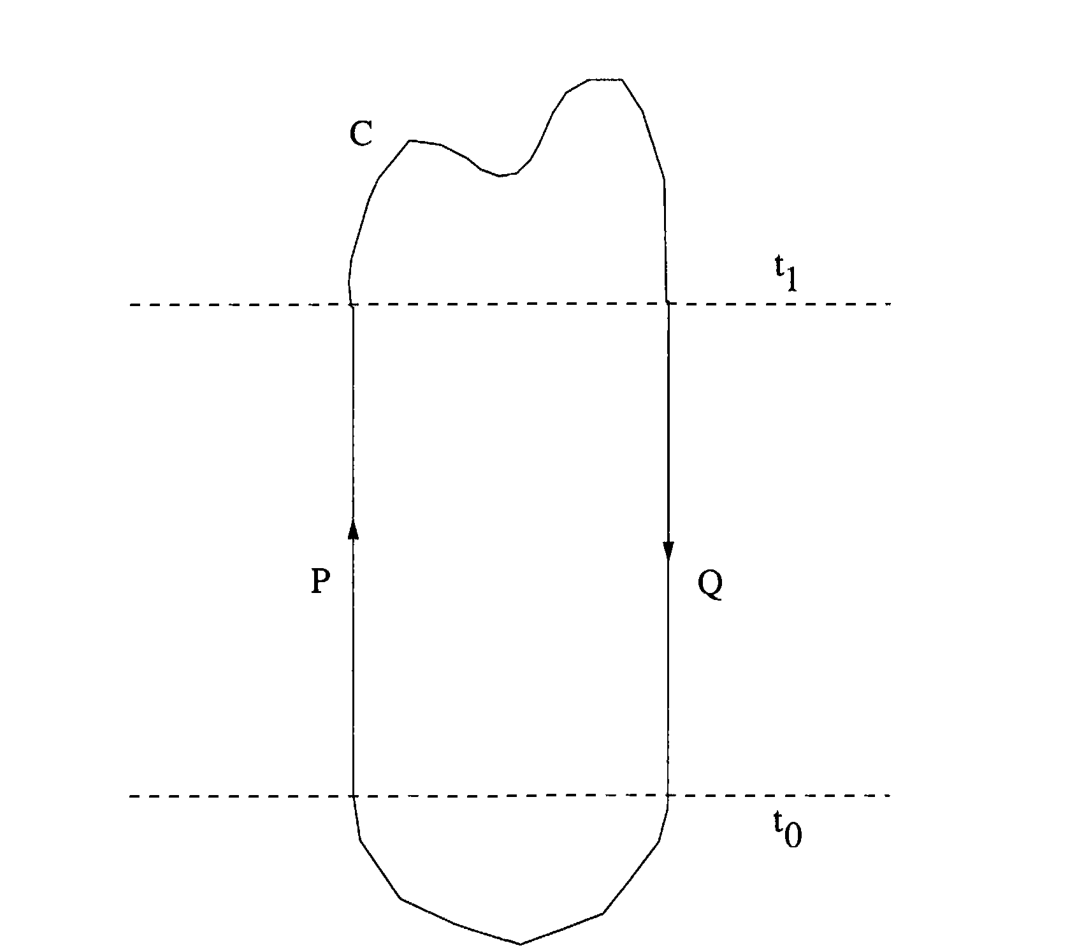
\includegraphics[width=0.52\textwidth]{figs/fig_p099_1.png}
  \caption{Wilson 圈 $C$ 的时空形状示意图。$C$ 在 $t_0<t<t_1$ 之间呈 $P\times\mathbb{R}-Q\times\mathbb{R}$ 的形状（沿 $P$ 一侧向上、沿 $Q$ 一侧向下，箭头表示定向），而在 $t_0$ 之前与 $t_1$ 之后被「封闭」起来；两条虚线是时刻 $t=t_0$ 与 $t=t_1$ 的空间切片。（原文 Figure 1，p.99）}
  \label{fig:p099-1}
\end{figure}

如本页图所示，我们假定：在某个时刻 $t_0$ 之前、以及在某个时刻 $t_1$ 之后，$C$ 并不只是看起来像 $P\times\mathbb{R}-Q\times\mathbb{R}$，而是以某种方式被「封闭」起来（closed off）。$t_0$ 之前的路径积分与 $t_1$ 之后的路径积分分别算出某个初始态与某个末态，记作 $|\psi_i\rangle$ 与 $|\psi_f\rangle$，它们属于 $\mathcal{H}_{P,Q}$。（当然，我们还不知道 $\mathcal{H}_{P,Q}$ 是什么。）从时刻 $t_0$ 到 $t_1$ 的传播给出一个因子 $e^{-iH_{P,Q}(t_1-t_0)}$（若采用欧氏号差（Euclidean signature），则为 $e^{-H_{P,Q}(t_1-t_0)}$）。于是图中 Wilson 线的期望值可以算作
\[
\langle\psi_f|e^{-H_{P,Q}(t_1-t_0)}|\psi_i\rangle .
\]

但 $\mathcal{H}_{P,Q}$ 与 $H_{P,Q}$ 究竟是什么？

首先，如果给定了联络（我们将假定它在 $t_0$ 与 $t_1$ 之间与时间无关），而人们想用刚写下的那类公式来计算 $W_R(C)$，该怎么做？这纯粹是经典数学的问题，并不真正涉及量子场论。人们自然会这样定义 $\mathcal{H}_{P,Q}$：它由 $R\otimes R^*$ 构成（$R^*$ 是 $R$ 的对偶），其中我们认为 $R$「生活」在 $P$ 处、$R^*$「生活」在 $Q$ 处。\footnote{更确切地说，规范场 $A$ 是主丛 $\mathcal{P}$ 上的联络，它在 $P$ 处或 $Q$ 处的纤维我们记作 $\mathcal{P}_P$ 或 $\mathcal{P}_Q$。我们把 $\mathcal{P}_P\times_G R$ 记作 $R$，把 $\mathcal{P}_Q\times_G R^*$ 记作 $R^*$。} 在 $t=t_0$ 之前的「过去」中，从 $Q$ 到 $P$ 的平行移动（parallel transport）决定了 $R\otimes R^*$ 中的一个向量 $|\psi_i\rangle$；同样，在 $t_1$ 之后的「未来」中，从 $P$ 回到 $Q$ 的平行移动给出同一空间中的向量 $|\psi_f\rangle$。现在假定在 $t_0$ 与 $t_1$ 之间联络与时间无关，其含义是：相对于某个平凡化（trivialization），它可以用一个与时间无关的一形式表示。那么我们可以写出
\[
W_R(C)=\langle\psi_f|e^{-iH_{P,Q}(t_1-t_0)}|\psi_i\rangle
\]
其中 $|\psi_i\rangle$ 与 $|\psi_f\rangle$ 就是刚才描述的 $R\otimes R^*$ 中的那两个向量，而 $H_{P,Q}$（它是作用在 $R$ 上的项与作用在 $R^*$ 上的项之和）依赖于 $t_0<t<t_1$ 时那个特定的与时间无关的联络。（事实上，$H_{P,Q}$ 由此联络在「时间」方向上的分量决定。）

因此，若规范场是固定的，则只要取 $\mathcal{H}_{P,Q}=R\otimes R^*$，我们就能得到所需形式的表示。那么，若把规范场按量子力学处理，又当如何？

% [Tutor Note: 这里把与 $R$ 相伴的丛仍记作 $R$、把与 $R^*$ 相伴的丛仍记作 $R^*$，是全文的记号滥用；但真正要留意的是 $P$ 与 $Q$ 两处的因子互为对偶这一点。原因是：在 $t_0<t<t_1$ 区间内，$C$ 沿 $P$ 一侧向上、沿 $Q$ 一侧向下，两段具有相反的定向，故量子化后 $A_0$ 在两因子上的作用相差一个符号，$H_{P,Q}$ 实际为 $A_0^{(R)}\otimes 1-1\otimes A_0^{(R^*)}$ 型的算符；若把两处都取成 $R$（而非 $R^*$），则「时间」方向的相位不会相消，得到的就不是 $\operatorname{Tr}_R$ 沿圈的和乐，而是 $\operatorname{Tr}_R\bigl(\mathrm{Hol}\cdot\mathrm{Hol}\bigr)$ 之类无意义的量。等价的说法是：沿闭合圈定向走一圈时，$R^*$ 上诱导的平行移动是 $R$ 上平行移动之逆。]

% ===== 原文 p.100 =====
我们回忆一下：若把规范场按量子力学处理而不出现 Wilson 线，该怎么做。如上面所述，此时令 $\mathcal{A}$ 为所有联络构成的空间，$\mathcal{H}_0$ 为 $\mathcal{A}$ 上的 $L^2$ 函数构成的空间。然后我们考虑规范群 $\widetilde{G}$ 在 $\mathcal{H}_0$ 上的作用。物理的 Hilbert 空间就是不变元构成的空间 $\mathcal{H}$，即 $\mathcal{H}=\mathcal{H}_0^{\widetilde{G}}$。

显然，我们必须把这两种构造「混合」起来。下述自然的混合方式，可以通过重新审视最初把路径积分与 Hamiltonian 联系起来的那些论证来加以论证。（另一种做法是：我在 §7.7 中勾画了另一条论证下述构造的进路之开端。）我们把 $\mathcal{H}_0$ 替换为 $\mathcal{H}_0\otimes R\otimes R^*$，并定义 $\mathcal{H}_{P,Q}=(\mathcal{H}_0\otimes R\otimes R^*)^{\widetilde{G}}$。至于 Hamiltonian $H_{P,Q}$，它形式上由同一个表达式给出，即
\[
\frac{e^2}{2}\int d^3x\operatorname{Tr}\bigl(-\delta^2/\delta A(x)^2\bigr)+\frac{2}{e^2}\int d^3x\operatorname{Tr}F^2 ,
\]
只不过现在是在 $\mathcal{H}_{P,Q}$ 中求值。

% [Tutor Note: 印出的两项系数不相称：动能项为 $e^2/2$，而磁能项为 $2/e^2$，二者之积恰为 $1$。按 (7.15) 的作用量 $S=\frac{1}{4e^2}\int\operatorname{Tr}F\wedge *F$ 作正则量子化（取 $\operatorname{Tr}T^aT^b=\frac12\delta^{ab}$），对称的标准形式是 $H=\frac{e^2}{2}\int\operatorname{Tr}\Pi_i^2+\frac{1}{2e^2}\int\operatorname{Tr}B_i^2$（$B_i=\frac12\epsilon_{ijk}F_{jk}$，$\Pi_i$ 为 $A_i$ 的共轭动量），两项之积为 $1/4$；印出的 $2/e^2$ 与之差 4 倍（若把 $\operatorname{Tr}$ 换成基础表示的归一化，则差 2 倍）。故此处疑为排印之误，也可能是 $\operatorname{Tr}$ 与 $A$ 采用了另一种归一化。要点在于：$e$ 只以「$e$ 与 $1/e$ 配对」的方式出现——$e\to0$ 时动能项（电场能）趋于零而磁能项发散，这才是下文把 $e$ 当作弱耦合参数的意义所在；切勿用印出的字面系数去核对数值因子。]

更一般地，给定任意一组点 $P_i\in M_s$（$i=1,\dots,n$）以及与之相伴的 $G$ 的表示 $R_i$，我们令 $R_i(P)=\mathcal{P}_{P_i}\times_G R_i$。然后定义 Hilbert 空间
\[
\mathcal{H}_{P_1,R_1;P_2,R_2;\dots;P_n,R_n}=\bigl(\mathcal{H}_0\otimes\textstyle\bigotimes_{i=1}^{n}R_i(P)\bigr)^{\widetilde{G}} .
\]
我们说这就是「在点 $P_i$ 处带有处于表示 $R_i$ 中的外源电荷（external charge）的理论的 Hilbert 空间」。

我们可以把这推广到诸 $P_i$ 的位置随时间变化的情形。例如，让我们回到与一个圆 $C$ 相联系的 Wilson 圈的情形。我们仍假定 $C$ 在点 $P,Q$ 处横截地（transversely）与 $t=0$ 切片相交，但不再假定 $C$ 在 $t=0$ 附近与时间无关。令 $P(t),Q(t)$ 为 $C$ 与给定时刻的切片随时间变化的交点。于是我们必须在随时间变化的 Hilbert 空间族
\[
\mathcal{H}(t)=\bigl(\mathcal{H}_0\otimes R(P(t))\otimes R^*(Q(t))\bigr)^{\widetilde{G}}
\]
中工作，它带有一个随时间变化的 Hamiltonian，并且（我们希望）还带有一个自然的联络。

% [Tutor Note: 上句中 $R_i(P)$ 的括号里写的是 $P$，下标却是 $P_i$，正确记号应为 $R_i(P_i)$；这处不一致在下文 $\mathcal{H}(t)$ 的写法（$R(P(t))$）中才自洽。另需注意：当 $P(t)$ 随时间移动时，$(R(P(t)))^{\widetilde{G}}$ 这类「逐时刻取不变子空间」的做法只有在诸 $R(P(t))$ 之间给定了自然的等变联络（即「随时间变化的 Hilbert 空间族上的联络」）时才有意义——作者自己用 「hopefully」 一词承认这一点尚未建立，这正是他随即转入 §7.7 的动机。]

% 原文 §7.7
\subsection{Wilson 线算符的路径积分表示}

把经典 Wilson 线泛函表示成一维路径积分是方便的。这样的表示将在本节导出。除此以外，这一表示还可以用来把上述对 $\mathcal{H}_{P,Q}$ 的描述之论证纳入一个完全标准的形式。

设 $R$ 是单紧 Lie 群（simple compact Lie group）$G$ 的一个不可约有限维表示。由 Borel–Weil 理论，我们可以把 $R$ 看作 $H^0(G/T,\mathcal{L}_R)$，其中 $\mathcal{L}_R$ 是某个全纯线丛（holomorphic line bundle）。丛 $\mathcal{L}_R$ 带有自然的 Hermitian 度量，因而带有自然的联络 $B$。对任意映射 $\phi:S^1\to G/T$，定义作用量
\[
I_R(\phi)=-\ln\operatorname{Hol}\bigl(\phi^*(B)\bigr)
\]
（Hol 指和乐）。数 $I_R$ 只定义到 $2\pi i n$，但 $e^{-I_R(\phi)}=\operatorname{Hol}(\phi^*(B))$ 是良定义的。

考虑路径积分
\begin{equation}
  \tag{7.10}
  \label{eq:7-10}
  \int D\phi\,e^{-I_R(\phi)} .
\end{equation}
它可以表示成如下形式
\begin{equation}
  \tag{7.11}
  \label{eq:7-11}
  \int D\phi\,e^{i\int_D\phi^*(F_B)} ,
\end{equation}
其中 $F_B$ 是 $B$ 的曲率，$D$ 是以 $S^1$ 的像为边界的圆盘。由这个路径积分定义的量子理论，就是带有零 Hamiltonian 的 Hilbert 空间 $R$（因为该路径积分在微分同胚（diffeomorphism）下不变）。

% ===== 原文 p.101 =====
现在设 $P$ 是圆上某个主 $G$-丛的全空间（total space），带有联络 $A$，并令 $P/T$ 为与之相伴的 $G/T$ 丛。由于 $\mathcal{L}$ 是 $G/T$ 上的 $G$-等变（$G$-equivariant）线丛，它定义了 $P$ 上的一个复线丛，我们把它记作 $\mathcal{L}_P$。$\mathcal{L}$ 上的 Hermitian 联络 $B$ 在竖直方向（沿 $P$ 的纤维）定义了 $\mathcal{L}_P$ 上的一个联络。这个联络可以借助联络 $A$ 自然地延拓为 $\mathcal{L}_P$ 上的联络 $B_P$：在 $P$ 平凡且 $A=0$ 的局部规范中，$B$ 按「常值路径是水平路径」这一条件延拓。

对 $P/T$ 的任意光滑截面（section）$\phi$，定义作用量
\begin{equation}
  \tag{7.12}
  \label{eq:7-12}
  I(\phi,A)=-\ln\operatorname{Hol}\bigl(\phi^*(B_P)\bigr) .
\end{equation}
和以前一样，$I$ 只定义到 $2\pi i n$。

令 $W_R(A)$ 表示 $A$ 沿该圆的和乐在 $R$ 中的迹。现在容易看出，泛函 $W_R(A)$ 有如下积分表示：
\begin{equation}
  \tag{7.13}
  \label{eq:7-13}
  W_R(A)=\int_{\phi\in\Gamma(P/T)}e^{-I(\phi,A)}\,D\phi .
\end{equation}

% [Tutor Note: 「现在容易看出」背后用了三件事：(1) Borel–Weil 定理给出 $H^0(G/T,\mathcal{L}_R)\cong R$，且其余上同调为零（Borel–Weil–Bott），这就是为什么只有不可约表示才出现、且 $\phi$ 的靶空间必须是旗流形 $G/T$；(2) 由 (7.11) 定义的量子理论 Hamiltonian 为零，故它在圆上的配分函数就是其 Hilbert 空间的维数 $\dim R$，插入 $A$ 之后则给出 $\operatorname{Tr}_R$ 的平行移动；(3) $I$ 只在模 $2\pi i$ 的意义下定义，故 $e^{-I}$ 是映射空间 $\Gamma(P/T)$ 上某个线丛的截面，「对 $\phi$ 的积分」严格说是对该线丛截面的积分（需要把 $D\phi$ 的测度与曲率 $F_B$ 一并理解），这也是为何 (7.13) 的右端在 $A$ 作大规范变换下仍良定义。]

现在设 $C$ 是 $M$ 中的一个圈，$A$ 是 $M$ 上主 $G$-丛 $P$ 中的联络。设 $f:S^1\to C$ 是一个参数化。于是有
\begin{equation}
  \tag{7.14}
  \label{eq:7-14}
  W_R(C)(A)=\int_{\phi\in\Gamma(f^*P/T)}e^{-I(\phi,f^*A)}\,D\phi .
\end{equation}

这给出了 Wilson 线算符的一个积分表示。这一表示使我们能把 $C$ 存在时的理论用路径积分表示出来，而这个路径积分完全是标准类型的，只除了一点：某些场遍布整个时空，而 $\phi$ 只在 $C$ 上有定义。例如，在纯规范理论（pure gauge theory）的情形，我们会写
\begin{equation}
  \tag{7.15}
  \label{eq:7-15}
  \int DA\,D\phi\,\exp\Bigl(-\frac{1}{4e^2}\int\operatorname{Tr}F\wedge *F-I(\phi,A|_C)\Bigr) .
\end{equation}

一旦这样做，若再考虑 $C$ 在 $t_0<t<t_1$ 与时间无关的情形，就可以用完全标准的技术引入 Hilbert 空间与 Hamiltonian。沿着这条路走，就能重新得到我先前陈述的对 $\mathcal{H}_{P,Q}$ 的描述。在此请读者把它作为一个练习来思考。基本上，$R$ 与 $R^*$ 来自对 $\phi$ 的量子化，而 $\mathcal{H}_0$ 来自对 $A$ 的量子化；而限制到 $\mathcal{H}_{P,Q}=(\mathcal{H}_0\otimes R\otimes R^*)^{\widetilde{G}}$，正是规范场论中限制到规范不变态的通常做法。

\textbf{评注（Remark）}。注意 (7.13)、(7.14) 的被积函数是一个 Abel 联络的和乐，因此它可以显式地算作曲率积分的指数。这样，我们就把圆上任一线性微分方程的单值（monodromy）表示成了对无穷多个辅助变量（auxiliary variable）的显式积分。经典分析中众所周知：这样的表示若只允许有限多个辅助变量，一般是做不到的；只有某些「超几何」型的特殊方程才可能。

% [Tutor Note: 原文此句作 「This, we have represented the monodromy…」，按文意为 「Thus」，属排印讹误（同页上文刚用过 「This gives an integral representation…」 作句首，疑为串行）。此处的「无穷多个辅助变量」指截面 $\phi$ 在 $C$ 上每一点、每一方向上的取值，即 $\Gamma(f^*P/T)$ 是一个无穷维空间；而「有限多个辅助变量不可能」正是线性微分方程理论中「超几何型方程的和乐构成可约/有限单值群」的另一说法（参见 hypergeometric equation 与 Riemann–Hilbert 问题的经典结果），作者并未在此给出证明，只作类比。]

% ===== 原文 p.102 =====
% 原文 §7.8
\subsection{Higgs 相与禁闭相}

我们现在在欧氏空间（Euclidean space）中工作。考虑一个近似为矩形的 Wilson 圈：两个电荷产生、彼此分开距离 $L$，在该距离上保持时间 $T\gg L$，然后彼此湮灭。（见图。）

\begin{figure}[htbp]
  \centering
  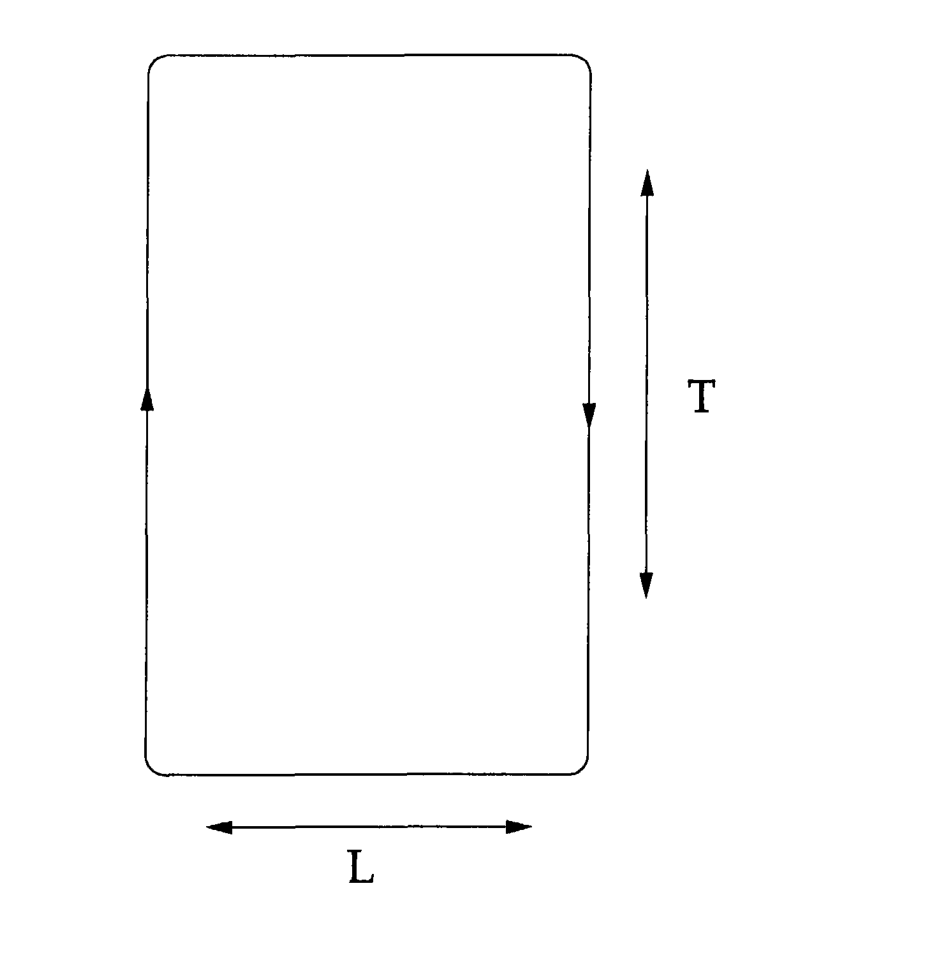
\includegraphics[width=0.42\textwidth]{figs/fig_p102_1.png}
  \caption{近似矩形的 Wilson 圈：纵向箭头标出 $T$（电荷对存在的时间），横向箭头标出 $L$（两电荷之间的距离）；左侧竖边上的箭头向上、右侧竖边上的箭头向下，表示 Wilson 圈的定向。（原文 Figure 1，p.102）}
  \label{fig:p102-1}
\end{figure}

于是 Wilson 圈算符的期望值 $\langle W_R(C)\rangle$（在欧氏框架下）有如下含义：它近似等于 $Ce^{-TV(L)}$，其中 $V(L)$ 是两个电荷在距离 $L$ 处的相互作用能量，而 $C$ 是一个依赖于 $C$ 在初始与末了时刻附近细节形状的常数。更确切地说，$V(L)$ 是 $\mathcal{H}_{P,Q}$ 中的基态能量与通常 Hilbert 空间 $\mathcal{H}$ 中的基态能量之差。关于 Wilson 圈期望值在 $T$ 很大时按 $Ce^{-TV(L)}$ 依赖于 $T$ 的断言，可由上面详细讨论过的它的 Hamiltonian 表示
\[
W_R(C)=\langle\psi_f|e^{-HT}|\psi_i\rangle
\]
推出。

% [Tutor Note: 此处的常数 $C$ 与圈 $C$ 同名，是原文的记号冲突（同一段中 $C$ 既指圈又指常数），阅读时须按上下文区分。另：由 $\langle\psi_f|e^{-HT}|\psi_i\rangle$ 看出，$e^{-TV(L)}$ 这一形式假定了 $T$ 远大于 $\mathcal{H}_{P,Q}$ 中第一激发态能隙的倒数 $\sim1/\Delta E$，从而只有基态存活；并且要求 $|\psi_i\rangle,|\psi_f\rangle$ 在基态上的投影不为零。因为该投影的绝对值被吸收进常数 $C$，所以 $C$ 依赖圈两端（即电荷「产生」与「湮灭」处）的形状，而不依赖 $T$、$L$。顺带一提，$V(L)$ 取的是「两态之「差」」，正是为了让 $V$ 中不含真空能密度这一发散量。]

所以 $\langle W_R(C)\rangle$ 的渐近行为取决于 $V(L)$ 在 $L\to\infty$ 时的渐近行为。物理学家相信，在二维以上具有质量间隙的规范场论中（二维有一些特殊性，其中一些我们稍后会看到），只有两种可能：

\begin{enumerate}
  \item \textbf{Higgs 相（Higgs regime）}：$V(L)\to\mathrm{const}$，$L\to\infty$。
  在这个相中，电荷（其类型见下面的评注）可以以有限的能量代价彼此分开。
  \item \textbf{禁闭相（confinement regime）}：$V(L)\sim\mathrm{const}\cdot L$，$L\to\infty$，其中该常数为正。
  在这个相中电荷被禁闭，不花费任意大的能量就不能彼此分开。
\end{enumerate}

现在让我们考虑任意形状的 Wilson 圈 $C$，其周长为 $S$，其所张成的曲面的极小面积为 $A$。有一个普遍的猜想：在给定质量间隙的前提下，若模式 1 与 2 在 $T\gg L\gg0$ 时成立，则它们对任意 $C$（在各个方向上都很大）以下述形式成立：Higgs 相对应于渐近行为 $\langle W_R(C)\rangle\sim e^{-wS}$（周长律（circumference law）），而禁闭相

% ===== 原文 p.103 =====
对应于渐近行为 $\langle W_R(C)\rangle\sim e^{-wA}$（面积律（area law））。在两种情形中，$w$ 都是正常数。

这一猜想背后的直观是：有了质量间隙，对 Wilson 线的响应或多或少是局域的——在 Higgs 情形中局域在 $C$ 本身上，在禁闭情形中则局域在 $C$ 所张成的极小面积曲面上。极小面积曲面是如何进来的，下周我们讨论 Polyakov 模型时会变得更清楚，随后在第 10 讲讨论 't Hooft 的禁闭图像时也会更清楚。

\textbf{评注 1（Remark 1）}。实际上，只有当 $R$ 是 $G$ 的万有覆盖（universal cover）$\widehat{G}$ 的表示、而不是 $G$ 本身的表示时，禁闭才可能发生。的确，若 $R$ 是 $G$ 的表示，则存在对 $\langle W_R(C)\rangle$ 有贡献的物理过程，其中 Wilson 线的很大一部分电荷为零（即携带 $G$ 的平凡表示），因为理论中某些粒子把 Wilson 线上的电荷湮灭了。这些过程的振幅大于面积律所预言的振幅。重要的是：上面模式 1 与 2 中讨论的「电荷」是借以探测理论的外源电荷——代价是把规范群 $G$ 换成它自己的一个覆盖。它们不是「原来」理论所描述的电荷；在有趣的情形中，它们甚至不像原来理论中的任何电荷那样变换。我们将在下面的玩具例子中说明这一评注。我预计这一评注难以理解，也不指望读者第一遍就能完全弄懂。

\textbf{评注 2（Remark 2）}。上面关于 Higgs 相与禁闭的判据 1 与 2，在其被定义的那类理论中是严格成立的。特别地，我们可以把周长律当作「一个有质量间隙的规范场论处于 Higgs 相」这一说法的精确陈述。这与我们在第 2 讲引入的 Higgs 机制密切相关，但并不总是完全一致。规范对称性破缺的微扰 Higgs 机制是一种在某些弱耦合理论中有用的计算方法。我们没有赋予它在弱耦合之外的意义（这与整体对称性的自发破缺不同——后者我们在第 1 讲给出了公理化的定义），而且即使在 $\pi_1(G)=0$ 时它也完全有意义（在这种情形下，由评注 1，我们目前这一更严格的讨论是空洞的）。相反，Higgs 相的周长律是一条支配某类有质量间隙理论的公理化判据；该判据的陈述与该理论是否有弱耦合描述、或与任何具体的计算方法都无关。按公理化判据处于 Higgs 相的理论，未必能用半经典 Higgs 机制描述（尽管在参数的某个极限下常常可以这样描述）；反之，由半经典 Higgs 机制支配的理论，按公理化判据也不总是处于 Higgs 相（尽管在实践中，当 $\pi_1(G)$ 非平凡时通常如此；事实上主要的反例就是我们即将描述的这个二维例子）。如果刚才这些论断现在显得令人困惑，读者应在进一步学习量子场论之后重新审视它们。

我们其实已经在第 5 讲讨论过禁闭的一个例子。作为另一个略有不同的玩具例子，让我们考虑拉格朗日量为 (7.1) 的二维理论，也就是本讲第一部分研究过的那个理论。此时 $G=U(1)$，其万有覆盖为 $\widehat{G}=\mathbb{R}$。设 $R$ 是 $\widehat{G}$ 的表示，由 $\lambda\in\mathbb{R}:x\mapsto e^{i\lambda x}$ 定义。于是，经典地有 $W_R(C)=e^{i\lambda\int_D F_A}$，其中 $\partial D=C$。

% [Tutor Note: 评注 1 的条件（$R$ 是 $G$ 的万有覆盖 $\widehat{G}$ 的表示而非 $G$ 的表示）与 p.105 猜想的条件（$R$ 不是伴随群 $G_{ad}$ 的表示）看上去互相冲突，实则针对两类不同理论：评注 1 讨论的是「含物质场」的理论，物质场本身取值于 $G$ 的表示，故任何一个 $G$ 的表示（哪怕高维）都可被「成对产生」的物质粒子完全屏蔽，只有不属于 $G$ 的表示（即 $G$ 的覆盖的表示）才无法屏蔽；而 p.105 讨论「纯规范理论」，此时能用来屏蔽的只有伴随表示中的胶子，它们保持电荷的「$N$-ality」不变，故只要 $R$ 不是 $G_{ad}$ 的表示（$N$-ality 非零）就无法屏蔽。对单连通的 $G$（如 $SU(3)$），$\widehat{G}=G$，评注 1 的条件确实空洞，这正是必须换成 $G_{ad}$ 的原因。换言之：评注 1 说的是「物质屏蔽」，猜想说的是「胶子屏蔽」，二者并不矛盾，但绝不可互相替代。]

% ===== 原文 p.104 =====
在量子力学上，我们可以写
\begin{equation}
  \tag{7.16}
  \label{eq:7-16}
  \langle W_R(C)\rangle=\int DA\,D\phi\,D\bar\phi\;e^{-\mathcal{L}}e^{i\lambda\int_D F} .
\end{equation}

% [Tutor Note: (7.16) 的指数写作 $e^{-\mathcal{L}}$，但 $\mathcal{L}$ 在 (7.1) 中是拉格朗日量「密度」，而此处需要的显然是欧氏作用量 $\int d^2x\,\mathcal{L}$（否则量纲与 (7.17) 中对 $V-A_C$、$A_C$ 的面积分解都无法对应）。这是作者一贯的记号滥用：本讲中他用 $\mathcal{L}$ 兼指密度与其积分。同理，$D\bar\phi$ 对应的复标量 $\bar\phi$ 在 (7.15) 中未写出（那里只写了 $D\phi$），因为 (7.15) 讨论的是纯规范理论、$\phi$ 是 Wilson 线的辅助场而非物质场，两者不可混淆。]

设 $V$ 是时空体积，$A_C$ 是 $C$ 所围的面积。我们将把路径积分 (7.16) 拆成两部分的乘积——对 $C$ 内部场取值的积分与对外部取值的积分。由于质量间隙，配分函数近似地分解为「内部」配分函数与「外部」配分函数之积。（还有一个在 $C$ 附近出现的周长修正；它不影响关于面积律的讨论。）注意 (7.16) 中最后一个因子（和乐因子）与 (7.1) 中的拓扑项属于同一类型。因此，(7.16) 给出
\begin{equation}
  \tag{7.17}
  \label{eq:7-17}
  \langle W_R(C)\rangle=\frac{1}{Z}\exp\bigl(-(V-A_C)E(\theta)-A_C E(\theta+2\pi\lambda)\bigr) ,
\end{equation}
略去边界项，我们在此不予考虑。这里 $E(\theta)$ 是作为 $\theta$ 的函数的真空能量密度；它可以用本讲第一部分的方法近似算出。由于在没有 Wilson 圈时配分函数为 $Z=e^{-VE(\theta)}$，我们得到
\begin{equation}
  \tag{7.18}
  \label{eq:7-18}
  \langle W_R(C)\rangle=\exp\bigl(A_C\bigl(E(\theta)-E(\theta+2\pi\lambda)\bigr)\bigr) .
\end{equation}

按照我们的计算，当 $\theta=0$ 时，$E(\theta+\lambda)-E(\theta)$ 化为
\begin{equation}
  \tag{7.19}
  \label{eq:7-19}
  E(\lambda)-E(0)=2(1-\cos2\pi\lambda)e^{-I/e^2}P .
\end{equation}

% [Tutor Note: 正文与 (7.19) 都写作 $E(\theta+\lambda)$、$E(\lambda)$，但按 (7.1) 的拓扑项 $-\frac{i\theta}{2\pi}\int F$，Wilson 圈因子 $e^{i\lambda\int_D F}$ 给出的平移量是 $2\pi\lambda$。用 (7.7) $E_{\rm vac}(\theta)=-P_0-2Pe^{-I}\cos\theta$ 直接验算：$E(2\pi\lambda)-E(0)=2Pe^{-I}(1-\cos2\pi\lambda)$，与 (7.19) 右端相符；而 $E(\lambda)-E(0)$ 只能给出 $1-\cos\lambda$，对不上。故 (7.19) 左端应为 $E(2\pi\lambda)-E(0)$，正文的 $E(\theta+\lambda)$ 应为 $E(\theta+2\pi\lambda)$——两处同样漏写了 $2\pi$；若把 (7.1) 的拓扑项误记成 $i\theta\int F$，则会得出「平移量就是 $\lambda$」的错误结论。(7.19) 中的 $P$ 是单瞬子行列式因子（见 (7.7) 与 §7.5）；另外本讲 (7.7) 写 $e^{-I}$、(7.19) 写 $e^{-I/e^2}$，同一量的两种写法前后不统一，读者应按「瞬子作用量 $=I/e^2$」理解。]

这总是正的，只要 $\lambda$ 不是整数。于是，$\theta=0$ 时的理论 (7.1) 对所有满足「$\lambda$ 不是整数」的外源电荷都表现出禁闭相。$\lambda$ 不为整数这一条件，意思不过是：我们出发时所用的表示是规范群的万有覆盖 $\mathbb{R}$ 的表示，而不是原规范群 $G=U(1)$ 的表示。这与上面的评注 1 一致：按我们所陈述的判据，禁闭只对这样的外源电荷出现——它们表示规范群的一个覆盖，而不表示规范群本身。

因此，尽管这个理论由微扰 Higgs 机制支配，按照上面的公理化判据，它在 $\theta=0$ 时处于禁闭相。所以在这个特例中，微扰 Higgs 机制与 Higgs 相的抽象判据相当不同。在二维以上，人们预期（并且在三维中已证明）这个理论按抽象判据也处于 Higgs 相，同时也表现出微扰 Higgs 机制。

回到二维，人们从上面还会看到：若 $\theta\neq0$，面积律中的系数可以是正的，也可以是负的。这是二维的一个奇特之处：在二维以上，负系数当然是不可预期的。

% 原文 §7.9
\subsection{禁闭猜想}

下面这个猜想在量子场论中是核心的。

% ===== 原文 p.105 =====
\textbf{猜想（Conjecture）}。\textit{设 $G$ 是单紧 Lie 群，$R$ 是 $G$ 的一个表示，且它不是伴随群（adjoint group）$G_{ad}$ 的表示。在 3 维与 4 维中，规范群为 $G$、拉格朗日量为 $\int\operatorname{Tr}(F\wedge *F)$ 的纯规范理论，对取值于 $R$ 的电荷表现出禁闭。在 4 维中，这对 $\theta$ 角的任何值仍然成立。}

这个猜想中与自然界观察到的强相互作用（它们支配核物理以及别的一些东西）相关的情形是 $G=SU(3)$、$R=\mathbb{C}^3$。该猜想的这一特殊情形就意味着夸克（quark）的禁闭。

在二维中，关于纯规范理论的类似陈述在 $\theta=0$ 时为真；这由我们第 5 讲的讨论可以推出。当 $\theta\neq0$ 时，二维的情形更复杂，即使在 Abel 情形中也是如此，正如我们刚刚所见。

\medskip
\noindent\textbf{参考文献与交叉引用（References and cross references）}

二维规范场论在第 5 讲与第 6 讲中讨论。Wilson 线算符以及 3 维、4 维中的禁闭在后面的讲次中讨论，特别是第 8 讲与第 10 讲。
